\documentclass{article}
\usepackage{fullpage}
\usepackage[T1]{fontenc}
\usepackage{titling}
\usepackage{graphicx}
\usepackage{enumitem}

\setlength{\droptitle}{-8em}   % This is your set screw
\title{Homework 2}
\date{}

\begin{document}
\maketitle

\section*{Instructions}
Read the given reading assignment and then attempt the problems.  Remember, for full
credit you must attempt all problems.  You must state the problem in your own words and show every step required to arrive at the solution.  Your work should be on a separate sheet of paper.  Do not turn in this assignment sheet with your homework.

\section*{Reading Assignment}
Read the following before attempting the problems in this assignment.  
Your quiz next Wednesday will include questions to test whether you read and studied
these texts.

\begin{itemize}
\item {\em A Treatise on Arithmetic} by J. Hamblin Smith. Chapter XXXI, Pages 241-250\newline
https://tinyurl.com/yb6c48ow\newline

\includegraphics[width=1in]{readings/treatise1}
\end{itemize}

\section*{Working With Formulae and Measurements}
For each of the following, carry out the required calculations.  Be sure to apply 
significant digits and rounding where appropriate.  The following formulae will help you:
\newline

\begin{tabular}{|c|c|c|c|}
\hline
Area of a Circle & Circumference of a Circle & Area of a Rectangle & Perimeter of a Rectangle\\
$A(r) = \pi r^2$ & $C(r) = 2\pi r$ & $A(l,w)=l \times w$ & $P(l,w) = 2\times l + 2 \times w$\\
\hline
\end{tabular}

\begin{enumerate}
\item You are planning to put new carpet on your living room floor.  Using a tape measure, you measure the width of the room to be $10.5\mathrm{ft}$ and the width measures $9.75\mathrm{ft}$.  How many square feet of carpet do you need to cover the floor?

\item Locate and measure each denomination of U.S. coin in common usage (penny, nickel, dime, and quarter).  What is the circumference and area of each, based on your measurement?

\item Stephen is a huge American football fan, so much so that he has decided to construct a football field in his own backyard.  The only problem he is having is the goal posts.  He needs to know how much pipe he needs to buy to construct the posts.  The dimensions and shape
of the goal is shown below.  For simplicity, we'll assume that Stephen is going to build the base straight up and down (and not using the curved neck usually seen in official fields.)
How much total pipe is needed to construct a single goal?\newline
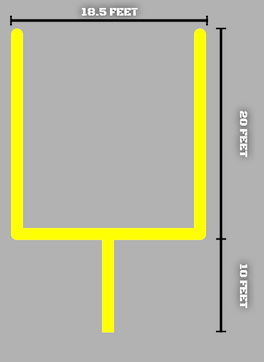
\includegraphics[width=2in]{images/football-goal}

\item Your grade in this class is computed as follows: Multiply your attendance average by 15, multiply your homework average by 5, multiply your quiz average by 15, multiply your project average by 30, multiply your regular exam average by 15, and multiply your comprehensive exam grade by 20.  Add all of these products together and divide by 100.  Write a function $g(a,h,q,p,e,c)=?$ which will compute your grade for the given average in each category.

\end{enumerate}

\section*{Ratio and Proportion}
\begin{enumerate}
   \item Arrange the numbers 4, 3, 9, and 12 into ratios so that they are in proportion.
   
   \item Divide \$1587 among four people (A, B, C, D) such that the ratio of A:B's share 
   is $6:5$, the ratio of B:C's share is $4:3$, and the ratio of C:D's share is $3:2$.
   
   \item Suppose a person pays income tax at the ratio of \$0.15 : \$1.00.  If their net 
   income (given by the formula $\mathrm{gross} - \mathrm{taxes}$) is \$15,215.00, what was their 
   gross income?
   
   \item Stephen's neighbors have learned about his football field idea and complained
   to the town council. Their key objection is that he is about to build a 
   30 foot tall structure out of steel pipe, and the town council agrees that this is an
   issue.  They inform Stephen that he may only build the structure to a height of 10 feet.  
   Undeterred, he decides he will build his goal posts, but he will comply with the law.  
   His idea is to build the goal posts to a height of 10 feet, but keep each of the
   dimensions in proportion to the original dimensions.  Draw a sketch of the new goal
   posts, labeling each of the dimensions for the shorter post. How much pipe will he
   need for his new goal post?
\end{enumerate}

\end{document}